\newpage
\section{Алгоритмы рисования диаграмм $k$-танглов}
	\label{section:drawing}

	Общая идея подобных алгоритмов рисования выглядит следующим образом: мы кодируем картинку конечным
	набором чисел, а затем сопоставляем каждой такой конфигурации числовое значение энергии с помощью
	некоторого выбираемого из эстетических соображений отображения. Затем с помощью какого-либо метода
	оптимизации мы находим изображение, соответствующее минимальной энергии --- это и будет результатом.

	Однако, чтобы получить картинки хорошего качества, надо использовать достаточно сложную функцию
	энергии, нахождение глобального минимума которой, вообще говоря, весьма нетривиальная задача. Еще одной
	проблемой является требование изотопности картинки изображаемой конфигурации --- со сложной
	функцией гарантировать его выполнение в глобальном минимуме практически невозможно. Поэтому мы будем
	строить изображение в две стадии --- сначала, используя максимально простую энергетическую функцию,
	получим начальное приближение, а потом, уже со сложной функцией, улучшим его методом градиентного
	спуска.

	\begin{figure}[ht]
		\centering
		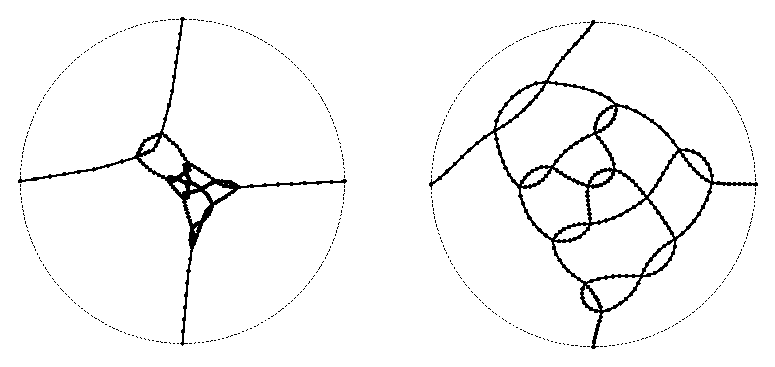
\includegraphics{c/drawing-energy.eps}
		\caption{Начальное приближение и градиентный спуск\label{figure:draw-optimization}}
	\end{figure}

	\subsection{Начальное приближение}

	На начальном этапе мы будем использовать простейшую возможную энергетическую функцию ---
	квадратичную форму
	$$
		E(x) = x \cdot Ax + b \cdot x
	$$
	Ее достоинствами являются простая физическая интерпретация как упругих взаимодействий и то, что минимум
	(если, конечно, он существует и единственен) легко найти из уравнения
	$$
		(A + A^T)x_{min} + b = 0
	$$

	Однако такой простейший подход, как выбрать в качестве переменных координаты перекрестков, а ребра представить
	упругими ``пружинками'' не приводит к желаемому результату (см.~\figureref{figure:degenerate-elastic}).
	\begin{figure}[ht]
		\centering
		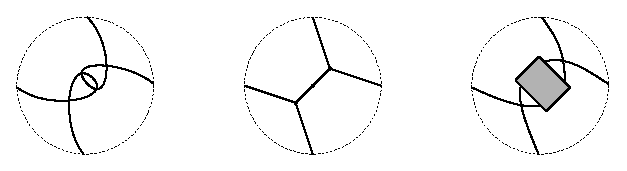
\includegraphics{c/drawing-initial-degeneration.eps}
		\caption{Диаграммы, вырождающиеся при утягивании\label{figure:degenerate-elastic}}
	\end{figure}

	Решить эту проблему можно при помощи добавления к графу дополнительных ребер-растяжек. Поместим в середину
	каждого исходного ребра тангла и каждой дуги границы-окружности дополнительный узел. Дополнительные узлы
	соединим между собой растяжками как показано на \figureref{figure:extra-elastic}. Можно представлять себе эти
	дополнительные ребра как стороны многоугольников, вписанных в грани исходного графа
	(\figureref{figure:extra-elastic}a), или же иначе --- как стяжки, попарно соединяющие соседние ребра, исходящие
	из каждой вершины тангла (\figureref{figure:extra-elastic}b).

	\begin{figure}[ht]
		\centering
		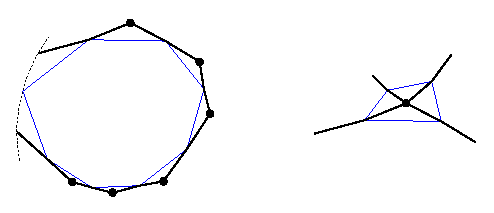
\includegraphics{c/drawing-face-crossing.eps}
		\caption{Дополнительные растяжки\label{figure:extra-elastic}}
	\end{figure}

	\begin{figure}[ht]
		\centering
		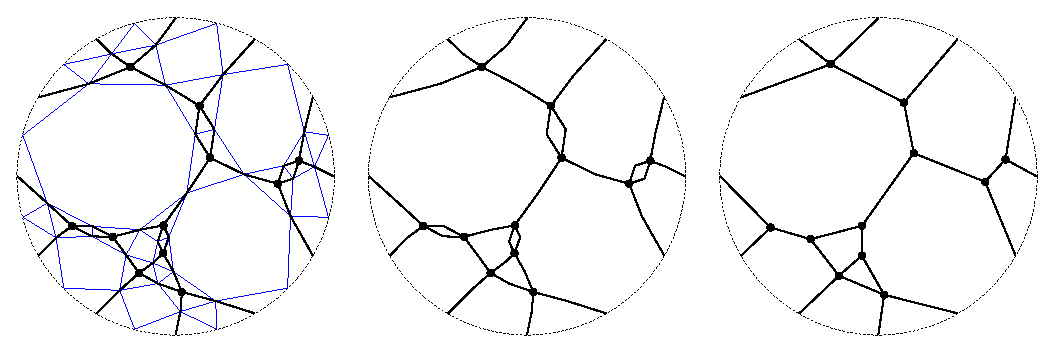
\includegraphics[scale=0.7]{c/drawing-initial-configuration-example.eps}
		\caption{Начальная конфигурация с растяжками и без\label{figure:startconfig}}
	\end{figure}

	При этом в каждой из 2-угольных граней мы получим две совпадающих растяжки. Оставим из них одну. Если у исходного
	тангла было $n$ перекрестков и $k$ концов, то полученный в результате граф содержит $n$ 4-валентных вершин
	(перекрестки исходного тангла), $k$ вершин валентности 2 (фиксированные дополнительные вершины на окружности)
	и $2n + k/2$ 5-6-валентных вершин (сколько ребер в графе тангла, 5-валентные вершины лежат на ребрах 2-угольных
	граней). Построим теперь для этого графа конфигурацию, соответствующую минимуму суммы квадратов длин ребер
	(см.~\figureref{figure:startconfig}).

	\subsection{Градиентный спуск}

	Второй стадией построения изображения, как и было сказано выше, является улучшение начальной конфигурации, полученной на
	предыдущем шаге. Для этого мы помещаем на каждом ребре начальной конфигурации еще по 1-2 промежуточных узла и запускаем
	метод градиентного спуска с новой более сложной энергетической функцией. В процессе мы должны следить за тем, чтобы за
	одну итерацию не происходило слишком больших прыжков, могущих изменить топологию текущей конфигурации, то есть ограничивать
	большие прыжки сверху.

	Основные требования к функционалу энергии для градиентного спуска:
	\begin{enumerate}
		\item
		бесконечный потенциальный барьер, препятствующий прохождению узлов через звенья;

		\item
		обращение в бесконечность при наложении ребер и стягивании в точку граней графа;

		\item
		непрерывность касательных в перекрестках;

		\item
		сходимость при увеличении числа точек на ребро;

		\item
		эстетические критерии --- хорошая различимость всех перекрестков и примерно равномерное распределение их в круге,
		длины ребер примерно равны, углы в перекрестках близки к прямым, плавное изменение кривизны
	\end{enumerate}

	Предлагаемая энергетическая функция будет линейной комбинацией четырех компонент: электростатического отталкивания элементов
	диаграммы друг от друга, электростатического отталкивания от граничной окружности, силы упругости ребер и ``изгибной''
	энергии, стремящейся спрямлять картинку в вершинах степени 2 и добиваться перпендикулярности входящих ребер в вершинах
	степени 4.

	Энергия электростатического отталкивания типа ``узел-узел'' не удовлетворяет самому важному требованию --- не обеспечивает
	потенциального барьера изменению топологии. Кроме того, рельеф потенциальной функции изобилует ямами. Энергия отталкивания
	типа ``звено-звено'' обеспечивает барьер, однако выражается довольно громоздкими формулами. Есть также проблема с вычислением
	сил взаимодействия сцепленных (инцидентных одной вершине) ребер. Наиболее подходящей кажется смешанная энергия ``звено-узел''.
	Будем считать, что заряд равномерно распределен по длине ребер тангла с единичной плотностью, но силы отталкивания сосредоточены
	в узлах, заряды которых пропорциональны полусумме длин соседних ребер. Такая схема соответствует вычислению повторного интеграла
	энергии при помощи смешанной квадратурной формулы --- одно интегрирование выполняется методом трапеций, а другое --- методом
	центральных прямоугольников.
	\begin{figure}[ht]
		\centering
		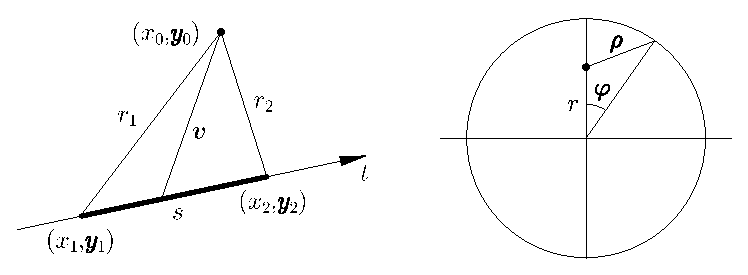
\includegraphics{c/drawing-energy-definition.eps}
		\caption{К определению электростатического потенциала взаимодействия\label{figure:electrostatic}}
	\end{figure}
	Электростатический потенциал, создаваемый заряженным отрезком (см.~\figureref{figure:electrostatic}):
	\begin{eqnarray*}
		\phi(x_0, y_0)
		= \int_0^s\frac{dt}{|\vec{v}|}
		= s\int_0^1\frac{d\tau}{\bigl([\xi_1(1-\tau)+\xi_2\tau]^2+[\eta_1(1-\tau)+\eta_2\tau]^2\bigr)^{1/2}} = {}\\
		= \ln\biggl(\frac{r_1+r_2+s}{r_1+r_2-s}\biggr)
	\end{eqnarray*}
	Здесь $\xi_{1,2}=x_0-x_{1,2}$, $\eta_{1,2}=y_0-y_{1,2}$; остальные обозначения приведены на~\figureref{figure:electrostatic}.

	Электростатический потенциал заряженной окружности единичного радиуса в ее плоскости (см.~~\figureref{figure:electrostatic}):
	$$
		\phi(r)=2\int_0^{\pi}\frac{d\phi}{\rho}=\frac{4}{1+r}\mathsf{K}\Bigl(\frac{4r}{(1+r)^2}\Bigr),
	$$
	где $\mathsf{K}()$ --- полный эллиптический интеграл 1-го рода.

	Изгибную энергию введем следующим образом. Для ломаной, заданной вершинами $p_k$, построим в каждой вершине векторы, равные
	сумме исходящих из данной вершины векторов звеньев (см.~\figureref{figure:bend-energy}). Определим изгибную энергию ломаной
	как сумму квадратов длин полученных векторов:
	$$
		E=\sum_k (x_{k-1}-2x_k+x_{k+1})^2+(y_{k-1}-2y_k+y_{k+1})^2
	$$
	Здесь $x_k$, $y_k$ --- координаты вершины $p_k$ ломаной.
	\begin{figure}[ht]
		\centering
		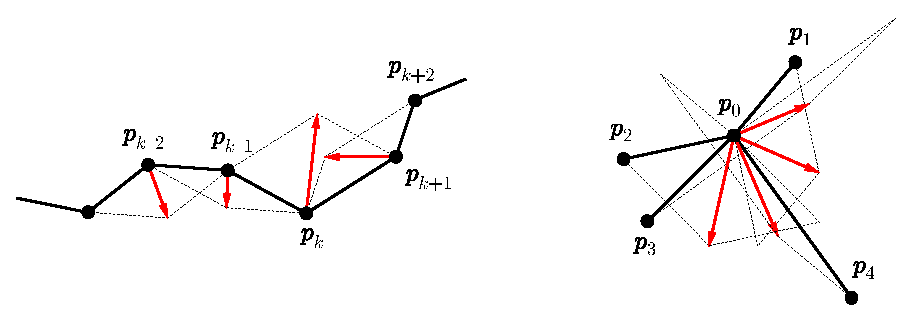
\includegraphics{c/drawing-bend-energy.eps}
		\caption{К определению изгибной энергии\label{figure:bend-energy}}
	\end{figure}
	Такая изгибная энергия равна нулю только для равнозвенной прямолинейной ломаной. Компоненты градиента изгибной энергии представляют
	собой разности 4-го порядка последовательности координат вершин:
	\begin{eqnarray*}
		\frac{\partial E}{\partial x_k} = x_{k-2} - 4x_{k-1} + 6x_k - 4x_{k+1} + x_{k+2} \\ [10pt]
		\frac{\partial E}{\partial y_k} = y_{k-2} - 4y_{k-1} + 6y_k - 4y_{k+1} + y_{k+2}
	\end{eqnarray*}

	Аналогичную функцию можно использовать для того чтобы выполнить еще одно требование к ``хорошо нарисованной'' проекции --- дуги в
	перекрестках должны пересекаться под приблизительно прямым углом. Обозначим узлы, соседние с данным перекрестком, в порядке против
	часовой стрелки, $p_1$, $p_2$, $p_3$ и $p_4$ (см.~\figureref{figure:bend-energy}) и введем соответствующие векторы, исходящие из
	перекрестка: $(x_1 - x_0, y_1 - y_0)$ и т.д. Мерой перпендикулярности двух последовательных векторов может служить вектор --- сумма
	одного из них с перпендикулярной копией второго. Энергию перекрестка определим как сумму квадратов длин таких векторов:
	\begin{eqnarray*}
		E = (x_2-x_0+y_1-y_0)^2 + (y_2-y_0-x_1+x_0)^2 + (x_3-x_0+y_2-y_0)^2 + \\
		+ (y_3-y_0-x_2+x_0)^2 + (x_4-x_0+y_3-y_0)^2 + (y_4-y_0-x_3+x_0)^2 + \\
		+ (x_1-x_0+y_4-y_0)^2 + (y_1-y_0-x_4+x_0)^2
	\end{eqnarray*}
	Это выражение обращается в ноль лишь когда все четыре вектора равны по величине, и все углы прямые.
